
Este capítulo apresenta o referencial teórico que fundamenta o desenvolvimento da plataforma. A Seção~\ref{sec:compiladores} discute a construção de compiladores e interpretadores, percorrendo as fases de análise léxica, sintática e semântica, a geração de código intermediário e objeto, as estratégias de otimização e a execução do código de máquina. A Seção~\ref{sec:engenharia-software} reúne as práticas de engenharia de software que orientaram o projeto: as metodologias ágeis de desenvolvimento, os testes automatizados, a separação de responsabilidades em camadas, as práticas de qualidade de código, a arquitetura do \textit{framework} Next.js e os princípios de Experiência do Usuário (UX) e Interface do Usuário (UI). Em seguida, são apresentados os softwares educativos e as tecnologias de apoio à aprendizagem e, por fim, os trabalhos relacionados, cuja análise crítica fundamenta o diferencial da solução proposta.

\section{Compiladores}
\label{sec:compiladores}

Esta seção percorre os fundamentos de compiladores que embasam o núcleo de tradução implementado neste trabalho, desde a definição de compilador e de suas fases até a geração de código intermediário.

\subsection{Compiladores e seus Fundamentos}

Um compilador é um programa cuja função é ler um código-fonte, escrito em uma linguagem específica, e traduzi-lo para um programa equivalente em uma linguagem-alvo. No modelo moderno de compilação, esse processo é estruturado em duas etapas principais e complementares: a análise e a síntese. A etapa de análise, comumente chamada de \textit{front-end}, divide o programa original em suas partes e gera uma representação intermediária do código. Por outro lado, a etapa de síntese, conhecida como \textit{back-end}, utiliza essa representação intermediária para construir e formatar o programa final desejado \cite{aho1995,cooper2012}.

Para facilitar a compreensão dessa separação lógica e visualizar a evolução da transformação do código, observe a Figura \ref{fig:fluxo_compilador}.

\begin{figure}[H]
    \centering
    \caption{Arquitetura de um compilador moderno.}
    \label{fig:fluxo_compilador}
    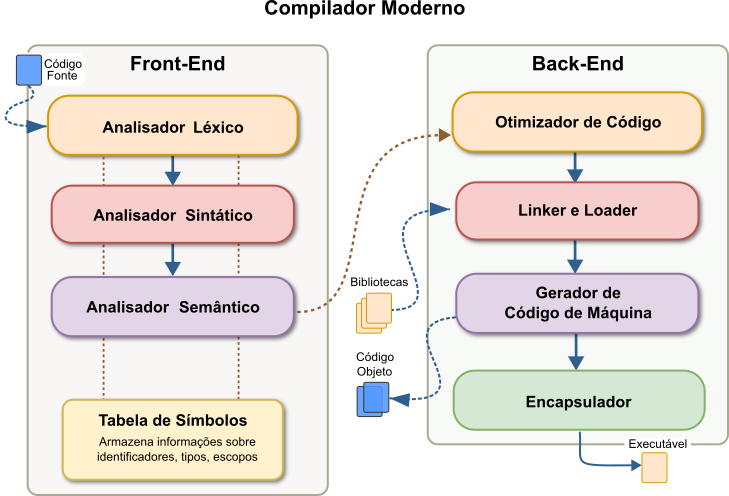
\includegraphics[width=0.8\textwidth]{Figuras/compiler.png}

    \legend{Fonte: \citeonline{alcantara2024}.}
\end{figure}

De modo conceitual, a operação de um compilador ocorre por meio de fases sequenciais, nas quais cada etapa tem o papel de converter o programa de um nível de abstração para outro. O núcleo de análise é formado pelas fases iniciais, que englobam as análises léxica, sintática e semântica. A partir desse ponto, o fluxo do compilador avança para as etapas de síntese, que englobam a geração do código intermediário, a otimização desse código e, por fim, a geração do código-alvo \cite{aho1995,cooper2012}.

A tabela de símbolos é gerenciada ao longo de todas essas fases. Trata-se de uma estrutura de dados muito importante para o compilador, pois mapeia todos os identificadores usados no programa fonte. Ao coletar e armazenar informações sobre os atributos de cada identificador, essa tabela permite recuperar escopos rapidamente e realizar a validação semântica durante a tradução \cite{aho1995,price2001}.

\subsection{O Modelo de Análise e Síntese (Fases da Compilação)}

De modo geral, a tradução é normalmente dividida em duas etapas principais: a análise e a síntese.
No estágio de análise (\textit{front-end}), o foco está em interpretar o programa original, dividindo-o em componentes menores para gerar uma abstração chamada representação intermediária.
Por outro lado, o estágio de síntese (\textit{back-end}) converte essa representação no programa final pretendido.
Essa distinção arquitetural entre \textit{front-end} e \textit{back-end} funciona como uma camada de abstração que simplifica a portabilidade, permitindo que o compilador suporte diversas linguagens e diferentes plataformas de hardware com maior agilidade \cite{aho1995,cooper2012}.

Para lidar com a complexidade da tradução de linguagens de alto nível, o fluxo operacional é dividido em unidades lógicas menores, chamadas de fases. Cada fase é responsável por uma transformação específica na representação do código. Na prática, essas fases podem ser agrupadas em ``passagens'' (\textit{passes}), estratégias que percorrem o código para otimizar a gerência de memória e o desempenho do sistema \cite{aho1995,cooper2012}.

As principais etapas que integram um compilador são detalhadas a seguir:

\begin{itemize}
    \item \textbf{Análise Léxica (\textit{Scanner}):} É a primeira etapa da compilação e processa o código-fonte caractere a caractere. Sua função é converter o fluxo de texto em uma sequência de unidades lógicas conhecidas como \textit{tokens}, removendo elementos irrelevantes para o processamento, como comentários e espaços redundantes \cite{cooper2012,nystrom2021}.

    \item \textbf{Análise Sintática (\textit{Parser}):} Utiliza a sequência de \textit{tokens} para validar a conformidade gramatical do programa em relação às regras da linguagem. O \textit{parser} organiza esses elementos em estruturas hierárquicas (as árvores sintáticas ou de derivação), empregando métodos descendentes (\textit{top-down}) ou redutivos (\textit{bottom-up}) \cite{aho1995,cooper2012}.

    \item \textbf{Análise Semântica:} Esta fase vai além da forma gramatical para garantir que as instruções tenham coerência lógica e operacional. Uma atividade importante aqui é a checagem de tipos (\textit{type checking}), que valida se a interação entre operadores, variáveis e funções respeita as definições da linguagem \cite{aho1995,cooper2012}.

    \item \textbf{Geração de Código Intermediário:} Concluídas as análises, o sistema produz uma versão do código que é independente da arquitetura final. O ``código de três endereços'' é um formato recorrente nesta etapa, servindo para reduzir a complexidade entre a abstração do alto nível e o rigor das instruções de máquina \cite{cooper2012,price2001}.

    \item \textbf{Otimização de Código:} Dedica-se ao refinamento do código intermediário, buscando torná-lo mais eficiente. O objetivo principal é reduzir o tempo de processamento e a ocupação de memória sem alterar o comportamento funcional do programa \cite{aho1995,cooper2012}.

    \item \textbf{Geração de Código Objeto:} Marca o encerramento da fase de síntese, na qual a representação intermediária é mapeada para a linguagem alvo (seja \textit{assembly} ou código de máquina). Esta etapa exige precisão na escolha das instruções nativas e cuidado na gestão dos registradores e endereços de memória do processador \cite{aho1995,cooper2012}.
\end{itemize}

Durante todo o ciclo, dois componentes dão suporte contínuo: o gerenciador da Tabela de Símbolos e o Tratador de Erros. A tabela de símbolos centraliza o registro de identificadores e seus metadados (como tipo e escopo), garantindo acesso rápido às informações em qualquer fase. Já o módulo de erros monitora falhas léxicas, sintáticas e lógicas, aplicando rotinas de recuperação que permitem ao compilador prosseguir com a análise e identificar o maior número possível de inconsistências em uma única execução \cite{aho1995,cooper2012}.

% ------------------------------------------------------------------------------------------------

\subsection{A Análise Léxica e o Reconhecimento de \textit{Tokens}}

Conhecida tecnicamente como \textit{scanner}, a análise léxica representa o estágio inicial do pipeline de compilação. Sua principal responsabilidade é percorrer o código-fonte caractere por caractere, processando essa entrada bruta para agrupar elementos em unidades com significado para a gramática da linguagem, chamadas de lexemas (conforme ilustrado na Figura \ref{fig:lexemas_nystrom}) \cite{cooper2012,nystrom2021}.

\begin{figure}[htb]
    \centering
    \caption{Exemplificação de agrupamento de caracteres em lexemas.}
    \label{fig:lexemas_nystrom}
    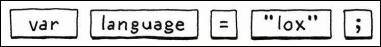
\includegraphics[width=0.8\textwidth]{Figuras/lex.png}
    \legend{Fonte: \citeonline[p. 43]{nystrom2021}.}
\end{figure}

Ao mesmo tempo em que organiza esses elementos, o analisador léxico realiza uma ``limpeza'' no fluxo de dados. Ele identifica e descarta componentes que, embora úteis ao programador, são irrelevantes para a tradução lógica, como comentários, tabulações e espaços em branco excedentes \cite{cooper2012,price2001}.

É importante, contudo, não confundir os conceitos de lexema e \textit{token}. O lexema refere-se à sequência literal de caracteres encontrada no texto original (a \textit{string} propriamente dita, como ``if'', ``soma'' ou ``42''). Já o \textit{token} é um objeto abstrato produzido pelo compilador para representar esse lexema. O \textit{token} carrega a categoria sintática da unidade (identificador, operador, palavra-chave) e, frequentemente, metadados adicionais, como o valor convertido e as coordenadas de linha e coluna, importantes para o rastreio de erros em fases posteriores \cite{cooper2012,nystrom2021}.

Para que o reconhecimento desses padrões ocorra de forma rigorosa, a micro-sintaxe da linguagem é definida por meio de expressões regulares. Esse modelo matemático permite descrever, de maneira concisa, as regras de formação de cada categoria de \textit{token}, definindo, por exemplo, quais combinações de símbolos formam um número real ou um nome de variável válido dentro daquela linguagem \cite{price2001,cooper2012}.

Contudo, expressões regulares são ferramentas de especificação, não de execução. Para que o computador processe essas regras, elas são convertidas em autômatos finitos. Um autômato funciona como uma máquina de estados: ele consome a entrada caractere por caractere, transitando entre estados lógicos até atingir um ``estado de aceitação''. Quando isso ocorre, o lexema é validado e o \textit{token} correspondente é enviado para o analisador sintático \cite{price2001,cooper2012}.

A implementação baseada em autômatos garante que a análise léxica seja eficiente, operando em tempo linear em relação ao volume de código. Na prática, desenvolvedores utilizam ferramentas de geração automática, como o \textit{Lex}, que transformam definições baseadas em expressões regulares diretamente em código otimizado de autômatos finitos determinísticos \cite{cooper2012,price2001}.

% ------------------------------------------------------------------------------------------------------------

\subsection{Estratégias de Análise Sintática: \textit{Top-Down} e \textit{Bottom-Up}}

A etapa de análise sintática, comumente chamada de \textit{parsing}, tem a tarefa de validar se a sequência de \textit{tokens} gerada previamente está de acordo com as regras gramaticais da linguagem de origem. Para processar essa estrutura e gerar a árvore de derivação, o sistema utiliza algoritmos baseados em duas abordagens principais: a análise descendente (\textit{top-down}), que atua da raiz para as folhas, e a análise ascendente (\textit{bottom-up}), que opera no sentido inverso \cite{aho1995,cooper2012}.

\noindent\textbf{I) Análise Sintática Descendente (\textit{Top-Down}):} Esta abordagem busca reconstruir a árvore sintática partindo do símbolo inicial (raiz) até alcançar os elementos terminais (folhas) que compõem o código de entrada. Durante esse fluxo, o analisador expande de forma sistemática o símbolo não-terminal posicionado mais à esquerda, utilizando as regras de produção para realizar o que se conhece tecnicamente como derivação à esquerda (\textit{leftmost derivation}) \cite{aho1995,price2001}.

Dentro dessa categoria, destacam-se os métodos recursivos descendentes e os preditivos baseados em tabelas, como o LL(1). O uso de analisadores por descida recursiva é frequente em projetos reais devido à sua legibilidade, simplicidade de implementação manual e eficiência no tratamento e diagnóstico de erros. Entretanto, para garantir um processamento linear e evitar o \textit{backtracking} (retrocesso), a gramática precisa ser cuidadosamente preparada: ela não deve apresentar recursão à esquerda e precisa ser devidamente fatorada. Isso assegura que o analisador consiga decidir qual regra aplicar consultando apenas o próximo \textit{token} da entrada \cite{cooper2012,nystrom2021}.

\noindent\textbf{II) Análise Sintática Ascendente ou Redutiva (\textit{Bottom-Up}):} Diferente do modelo anterior, a análise ascendente inicia o reconhecimento a partir dos \textit{tokens} individuais (folhas) e progride estruturalmente até atingir o símbolo inicial da gramática (raiz) \cite{aho1995,cooper2012}.

O termo ``redutiva'' caracteriza bem o funcionamento deste algoritmo: o analisador identifica padrões na pilha que correspondem ao lado direito de uma regra gramatical (denominados \textit{handles}) e os substitui (reduz) pelo respectivo símbolo não-terminal do lado esquerdo. Esse procedimento resulta em uma derivação à direita realizada de forma reversa \cite{aho1995,price2001}.

Os analisadores da família LR (como SLR, LALR e o LR Canônico) representam o que há de mais robusto nesta categoria, operando por meio de um sistema de empilhamento e redução (\textit{shift-reduce}) controlado por tabelas de estados. Uma vantagem significativa sobre a técnica descendente é a flexibilidade, pois os métodos \textit{bottom-up} lidam nativamente com recursão à esquerda e suportam quase todas as construções de gramáticas livres de contexto \cite{aho1995,cooper2012}.

Contudo, a criação manual das tabelas de transição para esses analisadores envolve alta complexidade matemática. Por esse motivo, a prática comum não envolve a codificação manual do \textit{parser}, mas sim o uso de ferramentas de geração automática, como o YACC, que traduzem a gramática formal diretamente em código funcional \cite{cooper2012,price2001}.

% -------------------------------------------------------------------------------------------------------------
\subsection{Análise Semântica e Verificação de Tipos}

Após a verificação gramatical feita pela análise sintática, o compilador entra na fase de análise semântica. Segundo \citeonline{price2001}, esta etapa tem como objetivo principal garantir que as estruturas e construções do programa, embora já validadas sintaticamente, façam sentido lógico para a posterior execução do código.
Enquanto o \textit{parser} (analisador sintático) assegura que a forma do código está correta, o analisador semântico vai além, inspecionando o que as peças do programa realmente significam de forma combinada \cite{nystrom2021}.
Nesse cenário, uma de suas atividades fundamentais é a resolução de associações, na qual o compilador verifica todas as variáveis mencionadas e determina exatamente a qual declaração de escopo cada identificador se refere \cite{nystrom2021}.

Outro componente central da análise semântica é a verificação de tipos \cite{aho1995, cooper2012}.
Nesta etapa, o compilador utiliza a estrutura hierárquica gerada previamente (a árvore de derivação) em conjunto com as informações coletadas na tabela de símbolos para checar se cada operador da linguagem está recebendo os operandos que lhe são legalmente permitidos \cite{aho1995}.
A análise semântica atua inferindo tipos para as expressões e detectando situações nas quais os valores são interpretados incorretamente \cite{cooper2012}.
Quando permitido pela especificação da linguagem, é também nesta fase que o compilador realiza conversões de tipo embutidas (coerções), como a transformação implícita de um valor inteiro para ponto flutuante antes de realizar uma adição entre tipos mistos \cite{aho1995, cooper2012}.

Os erros semânticos, por sua vez, são falhas peculiares, pois ocorrem em programas que podem possuir uma estrutura gramatical perfeitamente bem-formada, mas que violam as regras de significado, consistência ou contexto da linguagem de programação \cite{aho1995, cooper2012}.
O tratamento de erros semânticos é focado em capturar inconsistências que incluem, principalmente:

\begin{itemize}
    \item \textbf{Incompatibilidade de Tipos de Operandos:} Ocorre quando um operador é aplicado a um ou mais operandos cujos tipos de dados são conflitantes e não possuem regras de conversão implícita ou explícita \cite{aho1995, cooper2012}.
    Um exemplo prático na maioria das linguagens de programação fortemente tipadas é a tentativa inválida de se aplicar um operador aritmético binário a uma \textit{string} (texto) e a um booleano, ou tentar adicionar um tipo de precisão dupla a um tipo complexo de forma irregular \cite{cooper2012}.

    \item \textbf{Uso de Variáveis Não Declaradas ou Falhas de Escopo:} Este erro se manifesta quando o código faz referência a uma variável, função ou objeto que não foi previamente definido no programa, ou cuja declaração se encontra em um escopo léxico distinto e inacessível naquele momento \cite{cooper2012, nystrom2021}.
    A utilização de uma variável local fora de seu bloco restrito, por exemplo, acarretará uma falha semântica de identificador não reconhecido ou indefinido \cite{nystrom2021}.

    \item \textbf{Inconsistência de Aridade e Estruturas:} Acontece comumente em construções que exigem conformidade de números, como o número incorreto de argumentos \cite{cooper2012}.
    Exemplos incluem uma invocação de função ou chamada de procedimento na qual a quantidade de parâmetros passados difere da quantidade estipulada em sua definição original \cite{cooper2012, nystrom2021}.
    Igualmente, configura-se um erro semântico referenciar um \textit{array} informando um número de dimensões diferente do limite (ou \textit{rank}) estipulado em sua declaração \cite{cooper2012}.


\end{itemize}

% -------------------------------------------------------------------------------------------------------------

\subsection{Geração de Código Intermediário}

A fase de geração de código intermediário funciona como um mediador essencial entre a análise (\textit{front-end}) e a síntese (\textit{back-end}) de um sistema de compilação. Uma vez validadas as estruturas e a semântica do programa original, o compilador elabora uma representação interna explícita, projetada para ser agnóstica tanto em relação à linguagem de origem quanto à arquitetura de destino. Essa estratégia de tradução em múltiplos estágios é fundamental para decompor a complexidade de converter abstrações de alto nível em comandos de baixo nível de forma controlada. Além disso, essa camada de isolamento facilita a aplicação de técnicas de otimização e potencializa a portabilidade, visto que uma única representação interna pode ser mapeada para diferentes plataformas de \textit{hardware} \cite{cooper2012,price2001}.

Dentre os formatos de representação linear mais difundidos na literatura técnica, destaca-se o código de três endereços, que opera como um tipo de linguagem de montagem (\textit{assembly}) abstrata e universal. Nessa convenção, operações lógicas e aritméticas complexas são fragmentadas em instruções elementares contendo, no máximo, três operandos. A distinção crucial entre este formato e o código objeto final é que a representação intermediária ignora restrições físicas, como a gestão específica de registradores e o mapeamento direto de endereços de memória \cite{aho1995,cooper2012}.

Para exemplificar o conceito, considere uma expressão de atribuição como $A := X + Y * Z$. O compilador desmembra essa lógica em instruções de \textit{pseudo-assembly} simplificadas, utilizando variáveis temporárias para armazenar resultados parciais. O fluxo resultante em código de três endereços seguiria a sequência \cite{aho1995,cooper2012}:
\begin{enumerate}
    \item $T_1 := Y * Z$
    \item $T_2 := X + T_1$
    \item $A := T_2$
\end{enumerate}

A automação desse processo de conversão é viabilizada pela técnica de tradução dirigida pela sintaxe. Esse método expande o formalismo das gramáticas livres de contexto, permitindo que atributos sejam associados aos símbolos gramaticais e que ações semânticas específicas sejam vinculadas às regras de produção da linguagem \cite{aho1995,cooper2012}.

Na implementação prática, a emissão do código intermediário ocorre de forma síncrona com a análise sintática. No momento em que o \textit{parser} identifica uma construção gramatical legítima, ele dispara a ação semântica correspondente. Esse procedimento processa os atributos herdados ou sintetizados dos nós da árvore sintática, permitindo que os fragmentos de código sejam gerados de maneira ordenada e coerente com a lógica original do programa \cite{cooper2012,price2001}.

\subsection{Otimização de Código e Eficiência Computacional}

Posicionada estrategicamente como um estágio de refinamento no \textit{pipeline} de compilação, a otimização busca elevar a qualidade da representação interna do software. Esse aprimoramento vai além do ganho de velocidade e da economia de memória, abrangendo também a redução do consumo energético, um requisito crítico na computação contemporânea. Durante esta fase, o compilador atua substituindo construções genéricas por equivalentes semânticos mais ágeis. Um exemplo notório é o dobramento de constantes (\textit{constant folding}), que antecipa operações entre valores fixos ainda em tempo de compilação, eliminando o custo desse processamento durante a execução do programa \cite{aho1995,cooper2012}.

A legitimidade de qualquer transformação de código está condicionada a dois critérios imperativos: a preservação semântica (segurança) e a eficácia computacional (rentabilidade). O pilar da segurança determina que a lógica original do algoritmo deve permanecer inalterada, assegurando que a otimização não introduza efeitos colaterais. Já a rentabilidade exige que a alteração proporcione uma melhoria de desempenho real e mensurável, justificando o esforço computacional e o tempo adicional dedicados pelo compilador ao processo \cite{cooper2012,price2001}.

Quanto à abrangência das intervenções, a otimização é classificada em quatro níveis de profundidade:

\begin{itemize}
    \item \textbf{Otimização Local:} Restringe-se à análise de blocos básicos, isto é, sequências de instruções sem desvios de controle. Neste nível, utilizam-se frequentemente Grafos Acíclicos Dirigidos (GADs) para detectar e remover subexpressões redundantes e gerir variáveis locais de forma eficiente \cite{aho1995,cooper2012}.

    \item \textbf{Otimização Regional:} Expande o foco para conjuntos de blocos básicos, concentrando esforços prioritariamente em laços de repetição (\textit{loops}). Dado que a maior parte da carga de processamento ocorre nestes ciclos, melhorias como o deslocamento de código invariante geram impactos substanciais na performance global \cite{aho1995,cooper2012}.

    \item \textbf{Otimização Global (Intraprocedural):} Analisa o contexto integral de uma função ou procedimento. Por meio de estudos minuciosos do fluxo de dados, o compilador identifica oportunidades de simplificação que seriam invisíveis sob uma inspeção puramente local ou limitada \cite{aho1995,cooper2012}.

    \item \textbf{Otimização Interprocedural:} Atua no nível mais macro, transpondo as fronteiras entre diferentes módulos e sub-rotinas. Este escopo permite manobras agressivas como o \textit{inlining}, onde o corpo de uma função é integrado diretamente ao ponto de chamada, eliminando a sobrecarga (\textit{overhead}) associada ao desvio de execução e à gestão de pilhas de ativação \cite{aho1995,cooper2012}.
\end{itemize}

Na prática, a maioria das rotinas de otimização é dividida em duas etapas: uma fase de análise, dedicada ao mapeamento de dependências e do fluxo de controle, seguida por uma fase de transformação sintática, que efetivamente reescreve o código. Entre as técnicas mais usuais, destacam-se a eliminação de código morto (instruções inacessíveis ou inúteis), a simplificação de redundâncias aritméticas e a movimentação estratégica de cálculos para fora de zonas de alta repetição \cite{aho1995,cooper2012}.

\subsection{Geração de Código Objeto e Mapeamento de Arquitetura}

A fase de geração de código objeto (ou geração de código de máquina) representa a culminação do processo de compilação, consolidando as atividades finais do \textit{back-end}. O propósito central desta etapa é converter a representação intermediária otimizada na linguagem nativa da plataforma de destino. Para tanto, o compilador deve assegurar não apenas a fidelidade lógica em relação ao código original, mas também o aproveitamento máximo dos recursos de \textit{hardware} para garantir uma execução de alta performance \cite{aho1995,cooper2012}.

Um dos obstáculos primordiais nesta fase reside na acentuada heterogeneidade das arquiteturas de hardware. Cada família de processadores, a exemplo das arquiteturas x86, ARM ou RISC-V, possui sua própria Arquitetura do Conjunto de Instruções (ISA - \textit{Instruction Set Architecture}). Consequentemente, as operações de baixo nível e suas respectivas codificações binárias variam drasticamente entre diferentes sistemas, exigindo um mapeamento preciso para cada caso \cite{cooper2012,price2001}.

Para mitigar a complexidade de desenvolver um compilador do zero para cada novo processador, a engenharia de software moderna adota o princípio da \textit{retargetabilidade} (redirecionamento). Essa modularidade é viabilizada pelo papel central da representação intermediária: enquanto o \textit{front-end} opera de forma agnóstica em relação ao hardware, a adaptação para uma nova arquitetura exige apenas a substituição ou reconfiguração do módulo gerador de código (\textit{back-end}) \cite{aho1995,cooper2012}.

A síntese do código para uma máquina específica fundamenta-se em duas atividades interdependentes:

\begin{itemize}
    \item \textbf{Seleção de Instruções:} Atua como um mecanismo de reconhecimento de padrões que mapeia o fluxo do código intermediário para a sequência de comandos da ISA do processador que apresente o menor custo computacional possível \cite{aho1995,cooper2012}.
    \item \textbf{Alocação de Registradores:} Gerencia o conjunto limitado de registradores físicos da Unidade Central de Processamento (UCP). Esta tarefa é crítica, pois o compilador deve decidir estrategicamente quais valores devem permanecer nesses componentes de altíssima velocidade e quais devem ser transferidos para a memória principal (\textit{spilling}), visando minimizar os atrasos de acesso \cite{aho1995,cooper2012}.
\end{itemize}

% -----------------------------------------------------------------------------------------------------------
\subsection{Execução de Código de Máquina}

Ao término do processo de síntese, o que emerge é uma sucessão binária, densa e linear de operações primitivas. Diferente das abstrações hierárquicas manipuladas nas etapas iniciais da compilação, como as árvores sintáticas, o código de máquina é desprovido de estruturas de alto nível. Trata-se de uma linguagem de baixíssimo nível, constituída por instruções rudimentares que ocupam apenas alguns \textit{bytes} e ditam ações imediatas nos circuitos: movimentação de dados entre células de memória e registradores ou a execução de operações aritméticas básicas \cite{cooper2012,nystrom2021}.

Para que essa massa de dados binários ganhe vida, o programa deve ser transferido para a memória principal. Neste estágio, o sistema operacional, auxiliado por um \textit{software} carregador (\textit{loader}), prepara o ambiente de tempo de execução (\textit{runtime}). Este processo envolve a segmentação da memória em áreas distintas, isolando o setor de código estruturado das regiões destinadas ao armazenamento de dados \cite{cooper2012,price2001}.

A partir desse momento, o comando da execução passa à Unidade Central de Processamento (UCP). O ``guia'' dessa jornada é um registrador especializado da arquitetura, conhecido como Contador de Programa (\textit{Program Counter} - PC) ou Ponteiro de Instrução (\textit{Instruction Pointer} - IP), cuja função é monitorar rigorosamente o endereço da próxima instrução a ser processada \cite{cooper2012,price2001}.

A execução ocorre por meio de um ciclo mecânico e ininterrupto de busca e execução. O processador percorre a fita de instruções, decodifica o código de operação (\textit{opcode}) de cada entrada para extrair seu significado semântico e, em seguida, executa a tarefa correspondente. Nesse ecossistema de baixo nível, a complexidade dos laços de repetição e desvios condicionais das linguagens de alto nível é simplificada drasticamente. O controle do fluxo é resolvido exclusivamente através de operações de salto (\textit{jumps} ou \textit{branches}), que alteram o fluxo ao escrever um novo endereço de memória diretamente no Contador de Programa, desviando o ``foco'' da UCP de um ponto do binário para outro \cite{cooper2012,nystrom2021}.

%----------------------------------------------------------------------------------------------------------
\section{Engenharia de Software}
\label{sec:engenharia-software}

Esta seção reúne as práticas de engenharia de software que orientaram a construção da plataforma: a organização do trabalho em ciclos iterativos, a estratégia de testes automatizados, a separação de responsabilidades em camadas, as diretrizes de qualidade de código, a arquitetura do \textit{framework} adotado no \textit{front-end} e os princípios de experiência e interface do usuário.

\subsection{Desenvolvimento Iterativo e Incremental e \textit{Extreme Programming}}
\label{subsec:xp}

O gerenciamento clássico de projetos de software, frequentemente baseado no modelo em cascata (\textit{waterfall}), assume que o desenvolvimento pode ser tratado como uma sequência previsível e linear de atividades. No entanto, a engenharia de software lida com sistemas intrinsecamente complexos e com alto grau de incerteza, e o engessamento de requisitos em fases iniciais costuma resultar em desperdício e na entrega de produtos que não atendem às necessidades reais. Em contraponto a essa visão, o desenvolvimento iterativo e incremental assume a imprevisibilidade natural do processo e organiza o trabalho em ciclos curtos, nos quais o sistema cresce por acréscimos funcionais sucessivos, cada um integrado e verificado antes do início do seguinte \cite{agile2012,beck2004}.

Entre os métodos ágeis, o \textit{Extreme Programming} (XP) distingue-se por concentrar suas prescrições nas práticas técnicas de construção do software, e não em papéis ou cerimônias de gestão. O método parte do princípio de que o custo da mudança pode ser mantido baixo ao longo de todo o projeto, desde que o código permaneça simples, coberto por testes e continuamente refatorado. A mudança deixa, assim, de ser tratada como desvio a ser evitado e passa a ser incorporada ao fluxo normal de trabalho \cite{beck2004,wildt2015}.

As práticas que sustentam esse princípio incluem o planejamento incremental, no qual o escopo é detalhado apenas no momento em que será implementado; o \textit{design} simples, que evita antecipar estruturas ainda não exigidas; o desenvolvimento guiado por testes, que estabelece o comportamento esperado antes da implementação; a refatoração contínua, que preserva a legibilidade do código à medida que ele cresce; a integração contínua, que reduz o custo de reunir contribuições paralelas; e a propriedade coletiva do código, segundo a qual qualquer integrante pode alterar qualquer parte do sistema, sustentada pela revisão mútua entre os desenvolvedores \cite{beck2004,wildt2015}.

Essa combinação torna o XP particularmente adequado a equipes reduzidas, nas quais não há massa crítica para instanciar papéis especializados: os mesmos desenvolvedores acumulam as atribuições de levantamento de requisitos, projeto, implementação, teste e revisão. Nesse cenário, as práticas técnicas assumidas pelo método ocupam o lugar dos mecanismos de coordenação que métodos orientados a processo delegariam a papéis distintos \cite{wildt2015}. As subseções seguintes detalham três dessas práticas que estruturaram diretamente a construção da plataforma: os testes automatizados e o \textit{Test-Driven Development}, a separação de responsabilidades em camadas e as diretrizes de \textit{Clean Code}.

\subsection{Testes Automatizados e \textit{Test-Driven Development} (TDD)}
\label{subsec:testes-tdd}

A garantia da qualidade de um software exige validação contínua de seus comportamentos. Em projetos modernos, a automação de testes reduz a dependência de verificação manual e fornece uma rede de segurança para alterações, refatorações e evolução do código. Essa prevenção contra a quebra de comportamentos já consolidados é conhecida como teste de regressão; além de validar funcionalidades, os testes automatizados funcionam como documentação executável das regras de negócio do sistema \cite{aniche2012,silveira2012}.

Nesse contexto, o TDD inverte o ciclo tradicional de implementação, exigindo que o desenvolvedor escreva um teste automatizado antes da funcionalidade. O ciclo vermelho-verde-refatora consiste em criar primeiro um teste que falha, escrever o código mínimo para fazê-lo passar e, por fim, refatorar a solução mantendo o comportamento validado \cite{aniche2012,martin_coder}.

Mais do que uma técnica de verificação, o TDD também influencia o \textit{design} de software. Ao escrever o teste primeiro, o desenvolvedor precisa pensar na interface pública, nas dependências e na responsabilidade de cada componente; dificuldades excessivas na escrita dos testes podem indicar acoplamento elevado, baixa coesão ou problemas de arquitetura \cite{martin_clean,aniche2012}.

A estratégia de testes de um sistema costuma ser distribuída em diferentes níveis de granularidade, arranjo frequentemente ilustrado pela chamada pirâmide de testes. A base é composta pelos testes de unidade, rápidos e isolados, que verificam o comportamento de pequenas partes do código. O nível intermediário abriga os testes de integração, responsáveis por garantir a correta comunicação entre componentes e serviços de infraestrutura. No topo situam-se os testes de ponta a ponta (\textit{end-to-end}), que validam o sistema inteiro a partir da interface do usuário, ao custo de execuções mais lentas e frágeis. A recomendação decorrente é concentrar o maior volume de casos na base e reservar os níveis superiores para os fluxos mais críticos \cite{aniche2012,silveira2012}.

\subsection{Arquitetura Limpa e Separação de Responsabilidades}

O projeto arquitetural de um sistema deve separar responsabilidades em camadas com papéis independentes e bem definidos. A interface de usuário no \textit{front-end} concentra-se na experiência de uso e na integração visual, enquanto regras de negócio, persistência e serviços de apoio devem permanecer desacoplados de detalhes periféricos de entrega. Essa separação reduz dependências indevidas e facilita testes, manutenção e evolução do software \cite{martin_clean,silveira2012}.

No contexto da plataforma, a separação entre elementos de interface, regras de customização da linguagem, execução do código e persistência de dados contribui para que cada parte possa evoluir sem comprometer as demais. Essa organização também favorece o uso de padrões de projeto e abstrações voltadas à redução de acoplamento entre os módulos \cite{martin_clean}. Os padrões efetivamente adotados na construção da plataforma, bem como os pontos do código em que foram aplicados, são enumerados na Seção~\ref{sec:arquitetura-plataforma}.

\subsection{Qualidade de Código e \textit{Clean Code}}

A construção de um software de maneira ágil e sustentável esbarra invariavelmente na qualidade de sua base de código. O código-fonte é a linguagem formal na qual os requisitos de um sistema são expressos e detalhados de modo que a máquina possa executá-los. No entanto, sob a pressão de prazos, é comum que as equipes produzam códigos desorganizados, resultando em uma degradação estrutural contínua que, a longo prazo, faz a produtividade despencar, podendo até mesmo inviabilizar a evolução do projeto \cite{martin_clean_code,agile2012}.

Para combater essa entropia, a adoção das práticas de Código Limpo torna-se essencial. A escrita de um código limpo exige disciplina, o uso consciente de padrões e uma sensibilidade aguçada para reconhecer a desorganização e aplicar refatorações. Um código limpo deve ser elegante, simples, direto e, sobretudo, legível para os seres humanos. O profissionalismo no desenvolvimento de software pressupõe que o código não deve apenas funcionar, mas deve ser fácil de entender, alterar e estender por outros desenvolvedores \cite{martin_clean_code}.

Dentre as diretrizes estruturais básicas e inegociáveis para a manutenção dessa clareza na base de código, destacam-se \cite{martin_clean_code}:

\begin{itemize}
    \item \textbf{Nomes Significativos:} A nomenclatura de variáveis, funções, parâmetros e classes deve revelar claramente a sua intenção e responder ao porquê de sua existência e ao que o componente faz. Deve-se evitar o uso de siglas obscuras, codificações desnecessárias ou trocadilhos que exijam mapeamentos mentais, facilitando assim a leitura fluida e a busca no código \cite{martin_clean_code}.

    \item \textbf{Funções Pequenas e Focadas:} Uma função deve ser extremamente concisa e projetada para fazer estritamente uma única coisa, mantendo um único nível de abstração. Funções extensas que realizam múltiplas tarefas, agrupam várias seções lógicas ou que misturam tratamento de erros com a lógica de negócio violam a organização e dificultam o entendimento e a testabilidade \cite{martin_clean_code}.

    \item \textbf{Uso Consciente de Comentários:} O uso de comentários costuma compensar a incapacidade do programador de se expressar claramente através do próprio código. Eles não devem ser utilizados para encobrir ou justificar um código ruim ou confuso. A energia da equipe deve ser direcionada para tornar o código tão claro e autoexplicativo que elimine a necessidade de anotações redundantes \cite{martin_clean_code}.

    \item \textbf{Eliminação de Duplicidade e Refatoração contínua:} A repetição de código é o grande inimigo de um sistema bem desenvolvido, pois representa trabalho, risco e complexidade desnecessária. Deve-se melhorar o \textit{design} do código de forma contínua, aplicando refatorações que tornem o sistema mais enxuto e compreensível, sem alterar o seu comportamento externo \cite{martin_clean_code,agile2012}.
\end{itemize}

\subsection{O Framework Next.js e sua Arquitetura}

O Next.js é um \textit{framework} React voltado para a construção de aplicações web \textit{full-stack}, que facilita o desenvolvimento ao configurar internamente ferramentas de baixo nível, como empacotadores e compiladores, permitindo que o foco seja direcionado exclusivamente à construção do produto. A evolução de sua arquitetura ficou marcada pela transição do modelo tradicional de rotas, conhecido como \textit{Pages Router}, para o \textit{App Router}. Esse novo modelo adota uma arquitetura avançada centrada em \textit{React Server Components}, aprimorando o processo de busca de dados e permitindo o uso nativo de \textit{layouts} aninhados por meio de uma estrutura rigorosa de arquivos, utilizando convenções como \texttt{layout.tsx} e \texttt{loading.tsx} \cite{ziemann2025,vercel2024}.

A adoção de componentes de servidor transforma a forma de renderização, pois permite que o código seja executado exclusivamente no servidor e nunca seja enviado ao cliente, o que elimina a sobrecarga de arquivos JavaScript redundantes ao navegador. Integrado a essa estrutura arquitetural, o \textit{framework} disponibiliza o \textit{streaming}, uma técnica muitas vezes apoiada pelo \textit{React Suspense}, que permite enviar partes da interface gráfica progressivamente para o cliente à medida que os dados ficam prontos, reduzindo o tempo de espera inicial percebido pelo usuário \cite{lai2025,vercel2024}.

Outra característica de destaque, consolidada nas versões mais recentes, é o uso de \textit{Server Actions}. Tais ações consistem em funções assíncronas executadas diretamente no servidor que podem ser invocadas a partir de componentes interativos no cliente. Essa abordagem simplifica mutações de dados complexas, como submissões de formulários e interações com o banco de dados, eliminando a necessidade de criar arquivos manuais para \textit{endpoints} de API \cite{makerkit2026,vercel2024}.

Por fim, para a otimização em ambiente de produção, a ferramenta não apenas suporta múltiplas estratégias de renderização, como a estática e a dinâmica, mas também possibilita a escolha do ambiente de execução (\textit{runtime}) mais adequado para cada rota. O desenvolvedor pode optar pelo \textit{Node.js Runtime} padrão, que possui acesso completo a todas as APIs e ao ecossistema do Node.js, ou pelo \textit{Edge Runtime}, que opera com base em APIs da Web e é projetado para latência mínima e inicialização rápida ao lidar com lógicas de resposta simples \cite{makerkit2026,vercel2024}.

\subsection{Design de Experiência do Usuário (UX) e Interface do Usuário (UI)}
\label{subsec:uxui}

O \textit{design} de produtos digitais modernos compreende duas disciplinas fundamentais e complementares: a Experiência do Usuário (UX) e a Interface do Usuário (UI). A UX refere-se à percepção, às emoções e às respostas de um indivíduo ao interagir com um sistema ao longo de toda a sua jornada. Essa área vai muito além da usabilidade, englobando a compreensão profunda do comportamento, das necessidades e das frustrações do público-alvo. Para garantir uma boa experiência, a organização estrutural é essencial, sendo a Arquitetura da Informação a especialidade responsável por moldar, gerenciar e dispor os conteúdos de modo a tornar a navegação fluida, acessível e agradável \cite{seyffert2026,lima2024,raposo2012}.

Por outro lado, a UI diz respeito à camada visual e interativa com a qual o usuário interage diretamente. Isso inclui a definição rigorosa de leiautes, botões, tipografia, cores e componentes visuais. Mais do que atuar apenas na estética, uma interface bem projetada deve garantir clareza e consistência de uso. Uma organização confusa no aspecto visual pode comprometer toda a experiência global e levar ao abandono do sistema, independentemente de quão robusta seja a sua funcionalidade em \textit{back-end} \cite{seyffert2026,lima2024}.

A relação entre essas duas áreas é de forte complementaridade, na qual a UX estrutura a lógica e a solução do problema, enquanto a UI materializa essas soluções em uma interface tangível e eficiente. O desenvolvimento adequado em engenharia de software dita que a estruturação de UX anteceda a de UI; ou seja, define-se primeiramente quais problemas serão resolvidos e como os fluxos de navegação funcionarão, para somente então aplicar o \textit{design} visual \cite{seyffert2026,raposo2012}.

Essa intersecção técnica também é fortemente influenciada por aspectos cognitivos e leis da psicologia. O chamado ``efeito estética-usabilidade'', por exemplo, demonstra que os usuários tendem a perceber um \textit{design} esteticamente agradável, isto é, uma boa UI, como sendo inerentemente mais utilizável e eficiente na resolução de suas tarefas. Para avaliar e garantir a eficácia dessas interfaces, métodos de inspeção como a avaliação heurística são comumente aplicados. Trata-se de uma análise guiada por heurísticas (princípios gerais de bom \textit{design}) para certificar itens como a visibilidade do estado do sistema e a prevenção de erros, maximizando a usabilidade final do artefato \cite{yablonski2020,raposo2012}.

Um desdobramento operacional desses princípios é a acessibilidade da interface, normatizada pela especificação \textit{Accessible Rich Internet Applications} (WAI-ARIA), mantida pelo \textit{World Wide Web Consortium} \cite{w3c2023aria}. A especificação parte de uma constatação simples: os elementos nativos do HTML comunicam automaticamente seu significado às tecnologias assistivas, mas componentes ricos construídos com elementos genéricos (uma caixa de diálogo montada sobre \texttt{div}, por exemplo) chegam ao leitor de tela desprovidos de qualquer semântica. Para suprir essa lacuna, a WAI-ARIA define três categorias de atributos: os \textit{papéis} (\textit{roles}), que declaram o que um elemento é (diálogo, aba, menu, alerta); os \textit{estados}, que descrevem sua condição corrente e mutável (expandido, selecionado, desabilitado); e as \textit{propriedades}, que expressam relações estáveis entre elementos (qual rótulo descreve qual campo, qual região é controlada por qual botão). A especificação estabelece ainda requisitos de operação exclusivamente por teclado e de gerenciamento de foco, de modo que todo recurso acionável pelo ponteiro também o seja pela navegação sequencial, e que a posição do foco permaneça previsível quando a interface muda de estado \cite{w3c2023aria}.

\section{Softwares Educativos e Tecnologias de Apoio à Aprendizagem}

Uma plataforma educativa é um ambiente virtual desenvolvido para apoiar processos de ensino e aprendizagem, oferecendo recursos, ferramentas e conteúdos que facilitam a interação entre alunos, professores e instituições de ensino. Nesse cenário de transformação, a escolha da ferramenta certa não é apenas uma questão tecnológica, mas um fator determinante para o engajamento, a motivação e o sucesso educacional \cite{benedetti2025,mindmakers2025}.

Contudo, para aproveitar o potencial das novas tecnologias, a instituição de ensino precisa ir além da simples adoção de ferramentas digitais. É essencial entender o propósito pedagógico por trás de cada inovação, garantindo que a tecnologia esteja sempre a serviço da aprendizagem, e não o contrário. Afinal, a tecnologia educacional atua como um meio que exige professores preparados para usar recursos digitais de forma criativa e estratégica, conectando os alunos a um aprendizado relevante, dinâmico e significativo \cite{mindmakers2025}.

Quando projetada com esse foco pedagógico, uma plataforma educativa bem estruturada permite a personalização do aprendizado, ajustando-se ao ritmo e ao estilo de cada aluno, o que maximiza seu potencial e promove uma assimilação muito mais eficaz do conteúdo. Essa abordagem valoriza o tempo de cada estudante e amplia as suas capacidades ao longo de toda a jornada educacional. Ademais, a integração de dinâmicas interativas nas ferramentas de ensino, como a gamificação e a aprendizagem baseada em desafios, transforma a educação em um processo envolvente de recompensas. Esses sistemas lúdicos ajudam a despertar o interesse contínuo dos alunos e a desenvolver habilidades socioemocionais indispensáveis, como persistência e colaboração \cite{benedetti2025,mindmakers2025}.

\label{sec:softwares-apoio}

\section{Trabalhos Relacionados}
\label{sec:trabalhos-relacionados}

Esta seção tem como finalidade situar a plataforma desenvolvida neste trabalho no conjunto de soluções tecnológicas voltadas ao ensino introdutório de programação. Embora o objetivo do projeto seja apoiar a aprendizagem de programação, e não o ensino de construção de compiladores, sua própria natureza, a de uma IDE acoplada a um interpretador de gramática configurável, posiciona a proposta na fronteira entre dois universos de ferramentas: de um lado, os ambientes voltados à iniciação em programação; de outro, os projetos didáticos de construção de compiladores e de analisadores léxicos e sintáticos, cujas decisões técnicas e pedagógicas são pertinentes por dialogarem diretamente com o núcleo de tradução que sustenta esta plataforma. Por essa razão, são examinadas cinco iniciativas representativas do estado da arte, organizadas nas duas subseções seguintes conforme o grupo a que pertencem e observando, em cada uma delas, as escolhas de interface, os recursos pedagógicos e as estratégias de interação com o estudante. Ao final, apresenta-se uma análise comparativa que evidencia as lacunas restantes e o diferencial da abordagem proposta, que se situa justamente entre esses dois grupos.

\subsection{Ambientes Voltados à Iniciação em Programação}

Reúnem-se aqui as ferramentas cujo público-alvo é o estudante em primeiro contato com a programação e cujo propósito declarado é reduzir o atrito desse contato inicial. Cada uma é examinada segundo os três eixos anunciados no início desta seção: as escolhas de interface, os recursos pedagógicos e as estratégias de interação com o estudante.

\noindent\textbf{Portugol Studio e Portugol Webstudio}

\textit{Escolhas de interface.} Criado pelo Laboratório de Inovação Tecnológica na Educação (LITE) da Universidade do Vale do Itajaí, o Portugol Studio é distribuído como um ambiente de desenvolvimento integrado de código aberto, originalmente para instalação local. A migração posterior para o Portugol Webstudio transferiu edição, compilação e execução para o navegador, decisão que remove a barreira da instalação em laboratórios escolares com configurações heterogêneas. A composição da tela reproduz a organização convencional de uma IDE profissional, com editor central, painel de saída e área de inspeção, de modo que a familiaridade adquirida seja transferível a ferramentas de mercado \cite{gomes2020,univali2026}.

\textit{Recursos pedagógicos.} O recurso central é a própria linguagem: construções sintáticas inspiradas em C e PHP, porém com palavras-chave integralmente traduzidas para o português brasileiro, o que evita que o aprendiz lide com dois idiomas ao mesmo tempo durante o estudo das estruturas básicas de controle de fluxo e de dados. A esse núcleo somam-se um depurador com execução passo a passo, um inspetor de variáveis sincronizado com a linha em execução e uma árvore que representa a estrutura sintática do código produzido, recursos que tornam observável o que normalmente permanece implícito para o iniciante \cite{gomes2020,univali2026}.

\textit{Estratégias de interação.} A interação apoia-se na visualização do programa em funcionamento: o estudante acompanha, linha a linha, a alteração dos valores em memória, o que aproxima a execução mental do algoritmo de sua execução efetiva. O suporte nativo a bibliotecas gráficas e sonoras amplia essa estratégia ao permitir projetos lúdicos, como pequenos jogos, cuja saída visível fornece retorno imediato sobre o efeito do código escrito \cite{martins2025,univali2026}.

\noindent\textbf{Quorum: linguagem de programação baseada em evidências}

\textit{Escolhas de interface.} O ecossistema disponibiliza o Quorum Studio, IDE concebida desde o início para operar com leitores de tela, e não adaptada a eles posteriormente. O ambiente funciona tanto em modo \textit{offline}, com geração de \textit{bytecode} para a máquina virtual Java, quanto em modo executável no navegador, o que permite adotá-lo em contextos com restrições de instalação \cite{quorum2025,ladner2019}.

\textit{Recursos pedagógicos.} O traço distintivo do projeto é submeter as decisões de sintaxe e de semântica a verificação empírica, em vez de herdá-las por imitação ou familiaridade histórica. Os testes conduzidos pela equipe responsável compararam linguagens consolidadas no mercado a uma linguagem de controle cujas palavras-chave foram geradas aleatoriamente, recurso metodológico que isolou o efeito da forma sintática sobre o desempenho de novatos. As evidências indicaram que substituir símbolos como chaves, colchetes e pontos e vírgulas por palavras de vocabulário comum reduz de modo consistente as taxas de erro sintático, resultado visível em construções como \texttt{repeat 10 times}, cuja leitura se aproxima de uma instrução em linguagem natural \cite{stefik2013}.

\textit{Estratégias de interação.} A modalidade primária de interação prevista é auditiva: a linguagem foi desenhada para que sua leitura por síntese de voz permaneça inteligível, o que condiciona desde a escolha das palavras-chave até a pontuação. O ecossistema estende essa interação a domínios de saída variados --- áudio, gráficos e robótica ---, oferecendo ao estudante formas de perceber o resultado do programa que não dependem exclusivamente da leitura visual de texto \cite{quorum2025,ladner2019}.

\noindent\textbf{Beecrowd: prática de algoritmos e avaliação automatizada}

\textit{Escolhas de interface.} Antes denominada URI Online Judge, a Beecrowd é uma plataforma inteiramente web, organizada em torno de um catálogo de problemas navegável por tema e por nível de dificuldade. A interface não oferece ambiente de desenvolvimento: o estudante escreve a solução em ferramenta externa e submete o código pronto, o que pressupõe que ele já disponha de um ambiente configurado \cite{ferreira2025}.

\textit{Recursos pedagógicos.} O acervo contempla milhares de problemas categorizados, abrangendo desde estruturas básicas de seleção e repetição até tópicos avançados como grafos e programação dinâmica, e admite submissões em diversas linguagens consolidadas no mercado, incluindo C++, Python, Java e JavaScript. A graduação de dificuldade é o principal recurso didático, pois permite ao estudante progredir por incrementos e ao professor selecionar conjuntos coerentes com o momento da disciplina \cite{ferreira2025,maonocodigo2022}.

\textit{Estratégias de interação.} A dinâmica articula-se em torno de um ciclo curto de submissão e \textit{feedback}: o estudante lê o enunciado, redige uma solução e a envia ao sistema, que a executa contra um conjunto fechado de casos de teste e retorna, em poucos segundos, um veredito como ``\textit{Accepted}'', ``\textit{Wrong Answer}'' ou ``\textit{Presentation Error}''. Cabe observar que esse retorno é binário quanto ao resultado e não localiza o erro no código. Combinado a elementos de gamificação como \textit{rankings} públicos, fóruns e contagem de submissões aceitas, o ciclo sustenta um regime de prática deliberada que tende a manter o estudante em posição ativa \cite{ferreira2025,garcia2024}.

\subsection{Projetos Didáticos de Construção de Compiladores}

Reúnem-se aqui as iniciativas voltadas ao ensino da construção de tradutores. Embora se dirijam a um público mais avançado, suas decisões técnicas e pedagógicas dialogam diretamente com o núcleo de tradução que sustenta a plataforma proposta, e por isso são examinadas segundo os mesmos três eixos.

\noindent\textbf{Laila: gerador de analisadores léxicos e sintáticos \textit{online}}

\textit{Escolhas de interface.} A ferramenta oferece um ambiente de desenvolvimento inteiramente executado no navegador, construído em JavaScript com o \textit{framework} VueJS e apoiado na biblioteca CodeMirror, responsável pelo destaque de sintaxe e pela sinalização \textit{inline} de inconsistências. A camada de \textit{back-end} é uma API REST em Python que coordena a execução de FLEX e Bison no servidor. Essa escolha responde a um problema concreto de interface com a disciplina: a instalação coordenada desses geradores junto a uma cadeia compatível do GCC consome parte significativa da carga horária de laboratório, sobretudo em sistemas operacionais que não derivam do Linux \cite{ladgelson2021}.

\textit{Recursos pedagógicos.} O recurso didático central é a possibilidade de o estudante especificar gramáticas, redigir analisadores léxicos e sintáticos e executar os experimentos sem qualquer dependência local, concentrando o tempo de aula no objeto de estudo e não em sua configuração. O servidor captura comportamentos anômalos, como laços infinitos ou erros de compilação, e devolve os diagnósticos correspondentes ao cliente \cite{ladgelson2021}.

\textit{Estratégias de interação.} A interação organiza-se em um ciclo curto entre edição, submissão e retorno do resultado. Estudos de caso conduzidos junto a turmas de Ciência da Computação relataram ganhos perceptíveis de engajamento e de compreensão prática dos algoritmos de análise, atribuídos justamente à brevidade desse ciclo \cite{ladgelson2021}.

\noindent\textbf{\textit{chibicc}: abordagem incremental para o ensino de compiladores}

\textit{Escolhas de interface.} Este é o caso em que a análise por eixos revela a maior distância em relação às demais ferramentas: o \textit{chibicc} não possui interface própria. Trata-se de um repositório de código-fonte, cuja fruição pressupõe editor, cadeia de compilação e sistema de controle de versão já instalados e dominados pelo estudante. Toda a mediação recai sobre o histórico de \textit{commits} do projeto \cite{ueyama2020}.

\textit{Recursos pedagógicos.} O traço pedagógico mais relevante está na organização incremental. Em vez de expor o aprendiz, desde o princípio, a uma arquitetura completa com múltiplos passes e estruturas internas elaboradas, o projeto propõe uma trajetória gradual em que cada etapa adiciona uma única capacidade gramatical ou semântica ao compilador. O ponto de partida é um tradutor mínimo que reconhece apenas um número como entrada válida; sobre essa base, são integrados, em iterações sucessivas, suporte a expressões, declarações, controle de fluxo, ponteiros, estruturas e demais elementos do C11. Apesar do enfoque didático, o resultado cobre parte expressiva da especificação C11, sendo capaz de compilar, sem adaptações, projetos de complexidade considerável, como o sistema de controle de versão Git e o gerenciador de banco de dados SQLite \cite{ueyama2020}.

\textit{Estratégias de interação.} Não há retorno automatizado nem execução assistida: a interação consiste na leitura do código de cada etapa e em sua reimplementação pelo estudante, que verifica o próprio progresso executando manualmente a suíte de testes do projeto. A estratégia favorece a observação direta da relação entre escolhas de implementação e comportamento do compilador, mas transfere integralmente ao aprendiz a responsabilidade pela regulação do próprio ritmo \cite{ueyama2020}.

\subsection{Análise Crítica e o Diferencial da Solução Proposta}

A Tabela~\ref{tab:comparativo} sintetiza as principais características das ferramentas examinadas frente à plataforma proposta, evidenciando, em especial, a personalização da sintaxe pelo próprio estudante como traço distintivo da abordagem.

\begin{landscape}
\begin{table}[p]
    \centering
    \caption{Comparativo entre as ferramentas analisadas e a plataforma proposta, segundo os três eixos de análise.}
    \label{tab:comparativo}
    \footnotesize
    \setlength{\tabcolsep}{4pt}
    \renewcommand{\arraystretch}{1.3}
    \begin{tabular}{|>{\raggedright\arraybackslash}p{2.3cm}|>{\raggedright\arraybackslash}p{4.3cm}|>{\raggedright\arraybackslash}p{4.7cm}|>{\raggedright\arraybackslash}p{4.7cm}|>{\raggedright\arraybackslash}p{4.4cm}|}
        \hline
        \textbf{Ferramenta} & \textbf{Escolhas de interface} & \textbf{Recursos pedagógicos} & \textbf{Estratégias de interação} & \textbf{Personalização da sintaxe pelo estudante} \\
        \hline
        Portugol Studio e Webstudio
          & IDE própria, em versão local e em versão executada no navegador
          & Linguagem com palavras-chave em português; depurador, inspetor de variáveis e árvore sintática
          & Acompanhamento visual da execução; projetos gráficos e sonoros
          & Não \\
        \hline
        Quorum
          & IDE própria concebida para leitores de tela; execução local ou no navegador
          & Sintaxe definida por evidência empírica; operadores expressos por palavras
          & Leitura por síntese de voz; saídas em áudio, gráficos e robótica
          & Não \\
        \hline
        Beecrowd
          & Plataforma web sem ambiente de edição; exige ferramenta externa
          & Acervo graduado por tema e dificuldade; múltiplas linguagens de mercado
          & Ciclo submissão--veredito, sem localização do erro; gamificação
          & Não \\
        \hline
        Laila
          & IDE web com destaque de sintaxe e diagnóstico \textit{inline}
          & Dispensa a instalação de FLEX, Bison e GCC, liberando o tempo de laboratório
          & Ciclo curto entre edição, execução e diagnóstico
          & Sim, mas como objeto de estudo: o aluno escreve gramáticas formais \\
        \hline
        \textit{chibicc}
          & Sem interface própria; repositório de código-fonte
          & Trajetória incremental, uma capacidade da linguagem por etapa
          & Leitura e reimplementação do código; sem retorno automatizado
          & Não \\
        \hline
        \textbf{Plataforma proposta}
          & IDE web própria, com terminal integrado e sistema de arquivos
          & Exposição das fases de tradução (\textit{tokens} e código intermediário); avaliação automatizada de exercícios
          & Execução e depuração passo a passo; erros relatados no vocabulário escolhido pelo próprio estudante
          & Sim: palavras-chave, delimitadores de bloco, operadores, literais booleanos e terminador de instrução \\
        \hline
    \end{tabular}
    \legend{Fonte: elaborado pelo autor.}
\end{table}
\end{landscape}

Quando observadas em conjunto, as ferramentas analisadas organizam-se em dois grandes grupos cujas limitações afetam diretamente o público iniciante. O primeiro grupo reúne soluções dedicadas à prática algorítmica e à formação inicial em programação, do qual fazem parte o Portugol Studio, o Quorum e a Beecrowd. Embora apresentem avanços relevantes, seja por meio da tradução das palavras-chave para o português, da adoção de uma sintaxe baseada em evidências ou da prática contínua sustentada por avaliação automatizada, todas operam sob uma gramática fixa, definida previamente pelos seus responsáveis. O estudante permanece, portanto, na condição de quem se adapta à linguagem, e não de quem participa de sua modelagem; pequenas diferenças entre o vocabulário esperado e o vocabulário internalizado podem invalidar soluções logicamente corretas e reintroduzir, ainda que de forma reduzida, a barreira sintática que se buscava remover.

O segundo grupo reúne plataformas e projetos voltados ao ensino de compiladores propriamente dito, exemplificados pela Laila e pelo \textit{chibicc}. Ambos oferecem contribuições expressivas em seus nichos, sobretudo na eliminação do atrito de configuração ou na apresentação incremental da arquitetura de um compilador. Contudo, o público pressuposto é, em grande medida, o de estudantes em estágio avançado de cursos de Computação, com domínio prévio de linguagens estritas como C11 e de geradores como FLEX e Bison, o que afasta esses recursos do estudante que ainda enfrenta a barreira inicial de entrada no pensamento computacional.

A plataforma proposta situa-se entre esses dois grupos. Em vez de oferecer uma gramática previamente fixada ou de exigir a configuração local de cadeias de ferramentas, este trabalho disponibiliza uma IDE web integrada a um interpretador dinâmico cuja função principal é deslocar o controle estrutural da linguagem para o próprio estudante. Por meio da interface, é possível redefinir palavras-chave, delimitadores de bloco, operadores expressos por palavras, literais booleanos e regras de finalização de instrução, sem que o aprendiz precise lidar com a complexidade interna das fases de análise léxica, sintática e semântica.

Do ponto de vista da experiência do usuário, a personalização oferecida pela plataforma transforma o ato de programar em uma atividade na qual a linguagem se ajusta ao repertório do aprendiz, e não o contrário. Esse arranjo cria um laboratório seguro de experimentação algorítmica, no qual a frustração associada a erros de digitação ou de memorização de palavras reservadas é substituída pela investigação consciente das estruturas de controle e de dados. Forma-se, assim, uma ponte pedagógica entre a primeira aproximação ao raciocínio computacional e o futuro contato do estudante com as linguagens estritas e com os juízes automatizados que predominam no mercado e nas etapas mais avançadas da formação.
